% report.tex
% to compile, cd in your working dir, then use the command :
% "pdflatex report.tex" or "latexmk report.tex"
% and it shoul'd work
% in case of errors, type "X" to exit, correct your errors, and try again.
% NB: to update your table of contents, you need to compile twice !
% ask me anything if you need! (Josselin) OR look to this nice tutorial :
% https://en.wikibooks.org/wiki/LaTeX

% remember that you MUST escape all this caracters (with \) to visualize them :
% 			# $ % ^ & _ { } ~ \


\documentclass[a4paper,12pt]{article}

% utf-8 input:
\usepackage[utf8]{inputenc}

% for the margins of the document:
\usepackage[left=1.5cm,right=1.5cm,top=2cm,bottom=2cm]{geometry}

% to include graphics files:
\usepackage{graphicx}

% to do maths:
\usepackage{amsmath,amssymb}

% some meta-datas
\title{\textsc{Advanced Algorithmics Project:}\\Longest Common Subsequence}
\author{Edward Beeching\\Jérémie Blanchard\\Anthony Deveaux\\Josselin Marnat\\Joseph Renner}
\date{2016-2017}



\begin{document}
	\maketitle
	\newpage

	\renewcommand\contentsname{\begin{center}Table of Contents\end{center}}
	\tableofcontents

	\newpage
	\section*{Introduction}
		\paragraph{First paragraph} blablablabla

		
		\paragraph{itemized list}
			\begin{itemize}
				\item \textit{italic text}
				\item \textbf{bold text}
				\item \textsc{Text In Small Caps}
				\item \underline{underlined text}
			\end{itemize}

		\paragraph{numerized list}
			\begin{enumerate}
				\item bla
				\item blabla
			\end{enumerate}

	\newpage
	\section{Algorithms presentation}
		\subsection{LCS}
			\subsubsection{Dynamic programming}
				\paragraph{first par.} blablabla \\
				line break
			\subsubsection{}

		\subsection{Printing Neatly}

	\newpage
	\section{Preprocessing technics}
	
	\newpage
	\section{Graphical User Interface}
		\subsection{LCS Unit}
		\begin{figure}[h] %h:here
			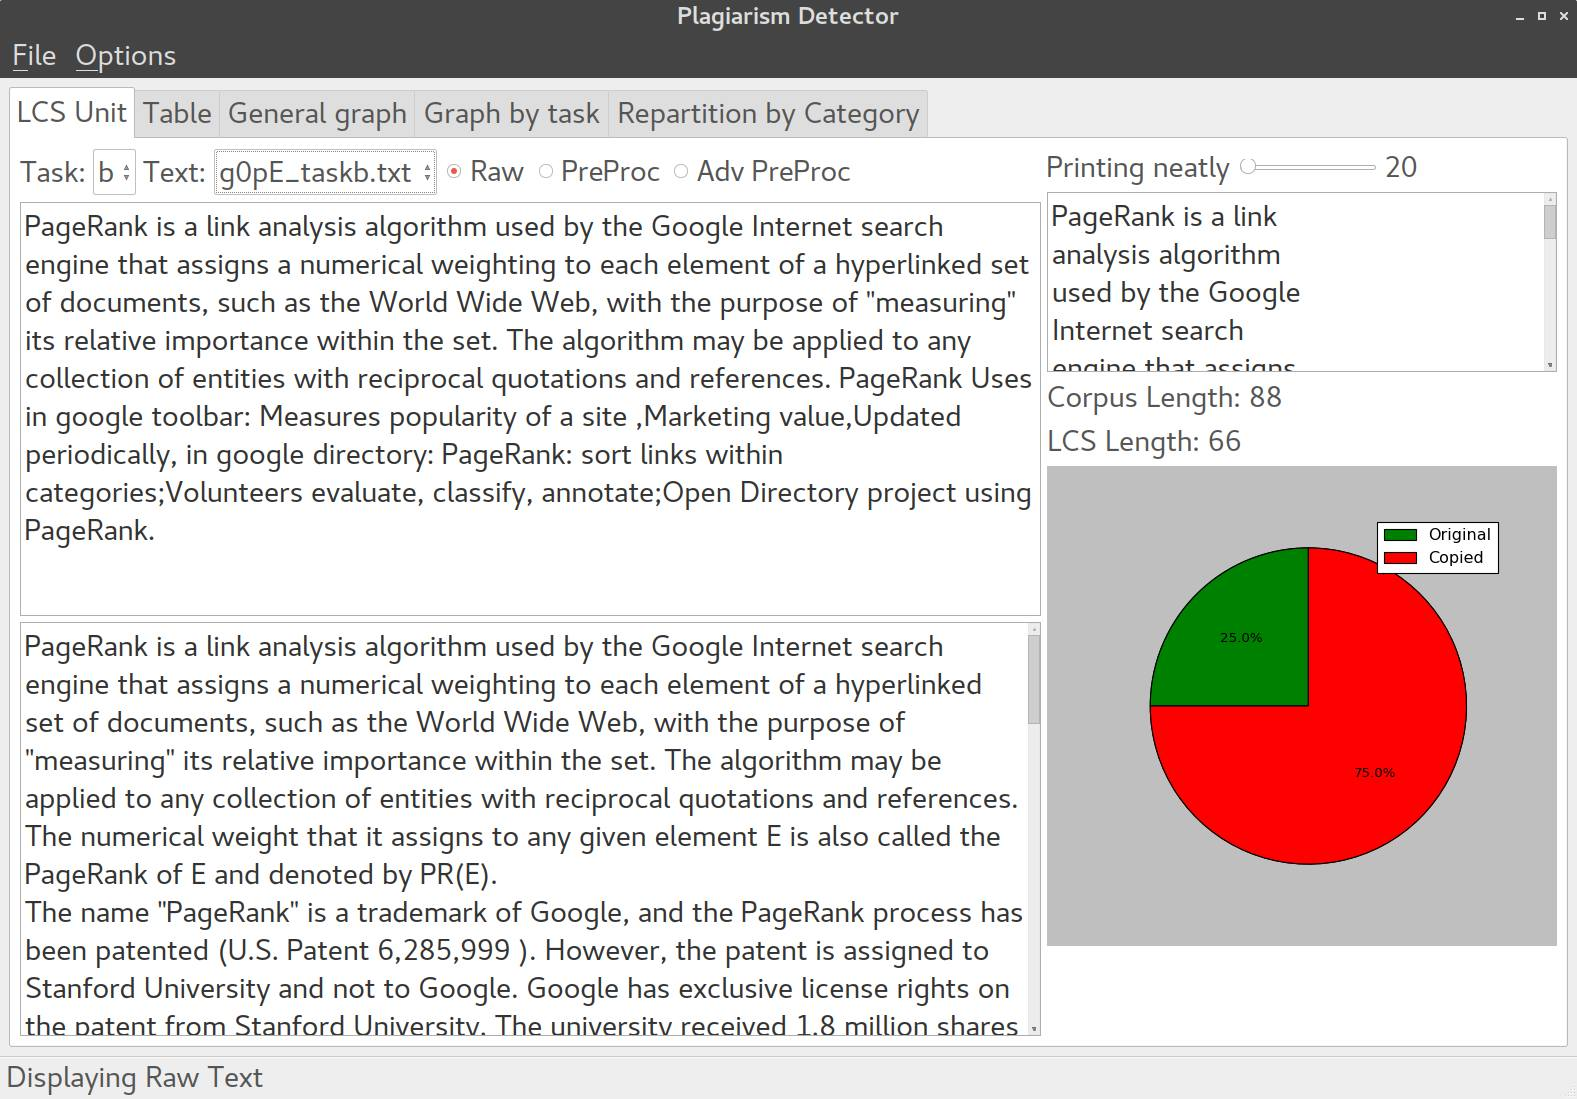
\includegraphics[width=10cm]{include/screen 1.jpg}
		\end{figure}

		\subsection{}

	\newpage
	\section{Results studies}
		\subsection{Time complexity}
			$$ \mathcal{O}_T = \text{some centered maths}$$
			We can also include maths inline the paragraph like $\sum_{i=1}^n \left[\sqrt{\frac{1}{\log{n^2}}}\right]$ or whatever.

		\subsection{Space complexity}
	
	\newpage
	\section*{Conclusion}

\end{document}
